% !TEX root = ../spec_kernel_agent_main.tex
\section{System Overview}\label{sec:overview}

\noindent\textbf{Overview.} We introduce \sysname{}, an agentic kernel
optimization system comprising \emph{SpecController} and
\emph{ElasticScheduler}.
SpecController utilizes the ongoing reasoning generation as a window for speculative
generation.
It forks non-reasoning generations conditioned on the reasoning prefix while
keeping the reasoning generation as a fallback.
Once a satisfactory kernel appears, SpecController terminates the
reasoning generation.
ElasticScheduler dynamically reallocates the validation/profiling resource pool,
prioritizes validation and profiling requests, and uses spare memory on
validation/profiling GPUs as remote KV-cache storage for reasoning prefixes.
\sysname{} requires \emph{no changes} to the underlying LLM or search algorithm.
It reduces generation latency, produces more profiling feedback, and keeps
validation/profiling resources busy.

\begin{figure}[t]
    \centering
    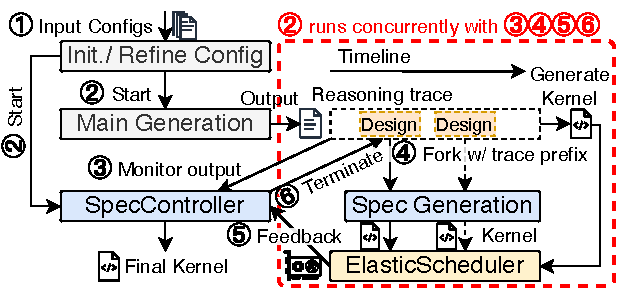
\includegraphics[width=\linewidth]{figs/Overview.pdf}
    \vspace{-20pt}
    \caption{System overview of \sysname{}.}
    \label{fig:system_overview}
    \vspace{-15pt}
\end{figure}

\noindent\textbf{Workflow.}\label{subsec:workflow}
One iteration of \sysname{} proceeds in the six steps below.
\noindent\textbf{(1) Input configuration.}
The user supplies three inputs: the reasoning LLM that will drive optimization,
the prompt template that describes the target kernel and feedback format, and
the search algorithm
(e.g., evolutionary search~\cite{AlphaEvolve,kernelagent2025,openevolve},
best-of-$N$~\cite{K-Search,cudaforge,TritonForge})
that governs how optimization status is updated between iterations.
Optionally, the user supplies a termination criterion for early stopping.
\noindent\textbf{(2) Start main generation and SpecController.}
\sysname{} starts the main reasoning generation.
At the same time, SpecController attaches to the main generation's reasoning output stream as a monitor.
The main generation remains live while steps~(3)--(6) execute, so these steps run concurrently with step~(2).
\noindent\textbf{(3) Monitor output.}
SpecController monitors the main generation's reasoning trace and detects
when the trace has committed to concrete kernel design, such as a tile-shape
choice, a parallelization plan, or a fenced CUDA code block.
These kernel-design decisions serve as trigger signals for non-reasoning
speculative generations.
\noindent\textbf{(4) Fork speculative generation.}
When SpecController emits a trigger signal, it concatenates the iteration's prompt
with the reasoning trace prefix to form a speculative prompt.
It forks speculative generations with this speculative prompt.
As each fork emits a candidate kernel, SpecController dispatches the kernel to
ElasticScheduler for validation and profiling.
SpecController maintains a history of kernels and their speedups to evaluate
the termination criterion.
\noindent\textbf{(5) Elastic scheduling for validation and profiling.}
ElasticScheduler receives validation/profiling requests from SpecController
and returns validation/profiling feedback to SpecController.
It dynamically partitions the GPU pool between validation and profiling to
absorb bursty arrivals, keep resources busy, and bound profiling feedback
latency.
\noindent\textbf{(6) Termination and output final kernel.}
SpecController analyzes the validation/profiling feedback to decide when to terminate the main reasoning.
If a speculative kernel meets the termination criterion, SpecController terminates the main generation and outputs this kernel as the final result.
If no early termination fires, the main reasoning generation remains a fallback,
and \sysname{} selects the best kernel found in the iteration.

% \noindent\textbf{How \sysname{} addresses the three inefficiencies.}\label{subsec:how_workflow_helps}
% The workflow above operationalizes the design insight of \S\ref{subsec:design_insight}.
% Step~(3) identifies useful prefixes from the streaming reasoning trace, and Step~(4) increases the candidate kernel count by forking non-reasoning generations while the main reasoning continues.
% Step~(5) validates and profiles these kernels before the main reasoning completes, raising the profiling feedback rate and keeping validation/profiling resources busy during generation.
% Step~(6) shortens the generation latency when a forked kernel meets the termination criterion; otherwise, it selects the fastest kernel produced within the current iteration as the final kernel.
% Together, these effects address the inefficiencies identified in \S\ref{sec:mot}.